\documentclass{subfiles}
\begin{document}

\subsection{Metodologie di Ricerca}
    Nello studio della personalità si muovono due concettualizzazioni generali: 

    \begin{itemize}
        \item Il primo punto di vista fa riferimento a un \textbf{approccio nomotetico} in cui 
        l'obiettivo del ricercatore è trovare delle regolarità, delle leggi nello studio della 
        personalità, applicabili a tutti. Esiste una predilezione per la raccolta e l'analisi di 
        dati più del tipo quantitativo con l'utilizzo di test uguali per tutti i partecipanti alla 
        ricerca.
        
        \item Il secondo punto di vista, è l'\textbf{approccio ideografico} in cui si privilegia 
        lo studio della singolarità della persona, con l'obiettivo di tracciarne un profilo unico 
        e particolare. Procedure di ricerca di natura prevalentemente qualitativa, come narrazioni 
        di vira del soggetto di studio. 
    \end{itemize}

    \subsubsection*{STUDIO DI CASI}
        Henry Murray (1938) conia il termine \textbf{personologia} per riferirsi allo studio 
        della persona come entità coerente ed unica (\textbf{ideografico}).

        Questo approccio ha consentito di promuovere una tecnica chiamata \textbf{studio di caso}, 
        ovvero uno studio intensivo e approfondito di una singola persona.
        Tale tecnica prevede un lungo periodo di osservazione e tipicamente include anche interviste 
        non strutturate.

        Questo studio permette di ottenere una grande quantità di informazioni relative alla 
        persona presa in esame, le quali vengono successivamente integrate per costruire dei 
        modelli dei comportamenti di quella persona nelle diverse situazioni.

        \begin{itemize}
            \item \textbf{\textsc{Vantaggi}}
            \begin{itemize}
                \item Conoscenza di aspetti intimi e complessi della vita del soggetto;
                \item Analisi di pensieri e sentimenti del soggetto in una data situazione;
                \item Unica fonte di dati per ricerca clinica
            \end{itemize}
            \item \textbf{\textsc{Limiti}}
            \begin{itemize}
                \item I risultati non sono generalizzabili;
                \item Il metodo non dimostra rapporti di causalità tra le variabili;
                \item Risente dell'interpretazione dello sperimentatore
            \end{itemize}
        \end{itemize}
        \clearpage

    \subsubsection*{LA RICERCA CORRELAZIONALE}
        Quando vengono elaborate le teorie o si traggono conclusioni dalle osservazioni, dovrebbero 
        poi poter essere applicate alla maggior parte delle persone o a tutte le persone, se possibile. 

        La \textbf{generalizzabilità} si riferisce al grado di applicabilità delle conclusioni di 
        una ricerca effettuata su in campione di persone all'intera popolazione da cui quel campione deriva. 

        La \textbf{ricerca correlazionale} prevede l'uso di questionari, nella maggior parte dei 
        casi di tipo self-report, che consentono di raccogliere molte informazioni su un ampio 
        numero di soggetti contemporaneamente.

        L'obiettivo è rilevare l'esistenza di una relazione tra due o più caratteristiche di 
        personalità, cioè la \textbf{correlazione} tra tali variabili. 

        Occorre misurare la \textbf{direzione} e la \textbf{forza} dell'associazione tra le variabili. 

        \textbf{ESEMPIO}: vogliamo capire come sono connesse tra loro l'autostima e il rendimento 
        scolastico.

        Misuriamo le variabili in un campione e otteniamo una distribuzione dei due punteggi che 
        rappresentiamo con un grafico di dispersione o \textbf{scatterplot}. (Figura \ref{fig:correlazione})

        \begin{figure}[h]
            \centering
            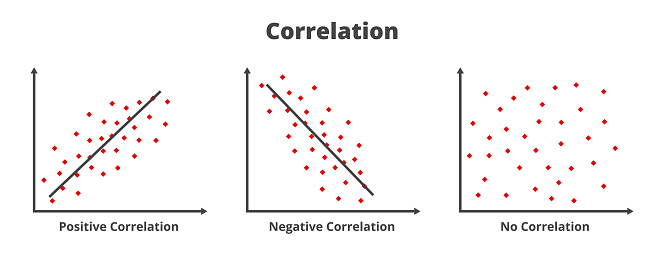
\includegraphics[width=0.5\linewidth]{correlation.png}
            \caption{\textbf{Direzione} dell'associazione tra le due variabili}
            \label{fig:correlazione}
        \end{figure}

        La \textbf{forza} dell'associazione tra le due variabili è il coefficiente di correlazione, 
        che varia da: 

        \begin{itemize}
            \item $+1.0$ (correlazione positiva perfetta) a $-1.0$ (correlazione negativa perfetta), 
            $0 =$ nessuna correlazione;
            \item valori tra $0.6 - 0.9$ indicano una forte correlazione;
            \item valori tra $0.3 - 0.5$ indicano una media correlazione;
            \item valori $< 0.3$ indicano una bassa correlazione.
        \end{itemize}

        \textbf{Limiti della Ricerca Correlazionale}
        \begin{enumerate}
            \item Non fornisce informazioni dettagliate come gli studi a caso singolo.
            \item Non consente spiegazioni di tipo causale tra le variabili esaminate, ovvero 
            perché due variabili sono associate.
            \item Risente dei limiti dei questionari di self-report, come l'acquiescenza e la 
            desiderabilità sociale.
        \end{enumerate}

    \subsubsection*{LA RICERCA SPERIMENTALE}
        La \textbf{causalità}, intesa come la relazione tra una causa e un effetto, ci informa del 
        `perchè' le variabili variano insieme.

        Nella correlazione tra autostima e rendimento scolastico, alta autostima potrebbe essere 
        la causa di alti rendimenti scolastici, oppure bassa autostima la causa di bassi rendimenti 
        scolastici. Potrebbe essere invece che alti rendimenti scolastici siano la causa dell'alta 
        autostima (bassa viceversa).
        Potrebbe entrare in gioco una terza variabile, non misurabile o non misurata (come il QI) 
        che abbia un rapporto causale con entrambe le variabili misurate. 

        La \textbf{ricerca sperimentale} è un approccio di ricerca i cui il ricercatore effettua 
        la manipolazione della \textbf{variabile indipendente}, assegna i partecipanti in maniera 
        casuale a una delle diverse condizioni sperimentali e, quindi, rileva l'effetto di tale 
        manipolazione sulla variabile dipendente. 

        Viene condotta un'indagine sperimentale per valutare l'impatto delle variabili in questione. 
        Questa metodologia implica un rigoroso \textbf{controllo} delle condizioni create 
        ad hoc, tra cui condizioni di successo o fallimento. I soggetti sono assegnati casualmente a 
        uno dei due gruppi di condizioni al fine di ridurre al minimo i potenziali bias. 
        Questa assegnazione casuale garantisce che ciascun gruppo abbia la stessa probabilità di 
        includere soggetti con caratteristiche simili, contribuendo così a controllare l'effetto 
        delle differenze individuali. La variabile dipendente, in questo caso l'autostima, viene 
        misurata attraverso un test self-report, il che consente di valutare in modo oggettivo 
        l'effetto delle condizioni sperimentali sui partecipanti.

        \textbf{Limiti della ricerca sperimentale} 
        \begin{enumerate}
            \item Molti comportamenti non possono essere studiati in laboratorio;
            \item Possono verificarsi varie distorsioni metodologiche:
            \begin{enumerate}
                \item effetti delle \textbf{caratteristiche della domanda} (intenzione e significato 
                della ricerca variano da individuo a individuo);
                \item effetti \textbf{aspettativa dello sperimentatore}.
            \end{enumerate}
        \end{enumerate}

        \subsubsection*{Quale tipo di ricerca è migliore?}
        Ogni approccio alla ricerca presenta vantaggi e svantaggi:

        \begin{center}
            \begin{tabular}{|m{5cm}| m{4cm} |m{4cm}|}
            \hline
            \textbf{Metodo} & \textbf{Vantaggi} & \textbf{Svantaggi}\\
            \hline
            \textbf{Studio di Caso} & comprensione profonda della persona. & le conclusioni non possono essere generalizzabili. \\
            \hline
            \textbf{Metodo Sperimentale} & mostra cause ed effetti. & incertezza su quale aspetto della manipolazione sia importante, esperimenti brevi in condizioni strettamente controllate.\\
            \hline
            \textbf{Metodo Correlazionale} & consente di esaminare eventi che si svolgono su lunghi periodi, consente di ottenere informazioni su eventi per i quali la manipolazione sperimentale non sarebbe etica. & non fornisce causalità.\\
            \hline
        \end{tabular}
        \end{center}
        

        \vspace{10pt}
        La \textbf{metodologia multi-metodo} o \textbf{pluralismo metodologico} consente di 
        integrare diversi metodi di ricerca per ottenere una conoscenza più precisa, completa e 
        sfaccettata della personalità stessa.

    \clearpage
\end{document}